\section{Étude théorique}
\subsection{La méthode TOFD}
\subsubsection{Principe du TOFD}

La méthode TOFD (\textit{Time Of Flight Diffraction}) a été proposée dans les années
1970~\autocite{bottcher_new_1973} ; les méthodes précédant TOFD étaient basées sur la
mesure de l'amplitude d'un signal réfléchi.
Celles-ci étaient peu fiables car les erreurs de calibration et l'orientation malheureuse de certains défauts pouvaient poser problème.

Au lieu de l'amplitude, la méthode TOFD se base sur la mesure du temps de vol d'une impulsion ultrasonore, afin de caractériser partiellement les défauts d'une pièce (par exemple des défauts de soudure).

La profondeur des défauts et leur étalement spatial peuvent être déterminés grâce à l'énergie diffractée.
Les avantages de cette méthode sont sa sensibilité et sa précision principalement ainsi que le fait qu'elle permette d'opérer un contrôle non-destructif. Avec l'utilisiation de TOFD les  composants les plus coûteux ont vu leur durée de vie rallongée car il est désormais plus facile d'analyser la fatigue de la pièce et d'en déduire le risque associé.

Expérimentalement, pour analyser une soudure, une paire de sondes à ultrasons est placée
de part et d'autre du cordon. La première sonde, l'émetteur, génère une impulsion qui est
ensuite captée par le récepteur, de l'autre côté de la zone à contrôler.

Cette technique utilise à la fois les ondes de volume mais aussi l'onde latérale générée lors de l'excitation. TOFD maximise ainsi le volume de matière couvert par l'inspection.
Lorsqu'un défaut est présent, l'onde ultrasonore est diffracté et le temps de vol modifié.
Grâce à un calcul trigonométrique simple, il est possible en utilisant le temps de vol de l'impulsion, de calculer la position du défaut.

Un schéma de principe de la méthode est disponible en Figure~\ref{fig:tofd_principe}.

\subsubsection{Matériaux controlés}

Le TOFD est principalement utilisé pour des matériaux peu diffusants. Par exemple il
peut-être utilisé pour des aciers possèdant des carbones non ou faiblement alliés.
Le problème des carbones fortement alliés (notamment dans l'acier inoxydable) est qu'ils
sont extrêmement diffractants, la détection du signal alors faible s'avère par conséquent
complexe.


\begin{figure*}[h]
    \centering
    \begin{tikzpicture}[>=stealth]
        % part
        \draw[very thick] (-5,0) -- (5,0);
        \draw[very thick] (-5,-2) -- (5,-2);
        \draw[very thick] (-5,0) .. controls (-6,-1) and (-4,-1) .. (-5,-2);
        \begin{scope}[shift={(10,0)}]
            \draw[very thick] (-5,0) .. controls (-6,-1) and (-4,-1) .. (-5,-2);
        \end{scope}

        % TX
        \newcommand\transducteur[1]{
        \draw (0,0) -- ++(2,0) -- ++(0,1.5) -- ++(-.5,0) -- ++(-1,-1) -- ++(-.5,0) --cycle;
        \begin{scope}[shift={(.65,.65)}, rotate=45]
            \draw (0,0) rectangle (.5,.7);
            \draw[thick] (.25,.7) .. controls (0,1.2) and (1,1.2) .. (.25,1.7);
        \end{scope}
        \draw[thin] (1.6,-.2) -- (1.6,1.7);

        % waves in plexi
        \begin{scope}[shift={(1,.5)}, rotate=-45]
            \draw[thick, #1, blue] (0.0) -- (.3,.1) -- (.4,0) --(0.7,.1);
        \end{scope}
				\draw[blue] (1.2, .7) node (l) {L};
        }
        \begin{scope}[shift={(-4.5,0)}]
					\transducteur{->};
				\end{scope}
        \begin{scope}[shift={(4.5,0)}, xscale=-1]
					\transducteur{<-};
				\end{scope}

        % waves in part
        \draw[thick, red, ->] (-2.5,-.3) -- ++(.9,-1.2) node[left] {TV};
        \draw[thick, red, ->] (-2.5,-.3) -- ++(1.2,-.9) node[above] {L};
        \draw[thick, red, ->] (-2.2,0) .. controls (-1.9,.3) and (-1.8,-.1) .. (-1.2,0) node[above] {Onde Latérale};

        % beams
        \draw[dashed, thin] (-2.9,0) -- ++(-25:4);
        \draw[dashed, thin] (2.9,0) -- ++(-155:4);
        \draw[dotted, thin] (0,-1.35) -- ++(5.5,0);
        \draw[dotted, thin] (5,0) -- ++(.5,0);
        \draw[<->] (5.4,0) -- ++(0,-1.35) node[midway, right] {$\nicefrac{2e}{3}$};
    \end{tikzpicture}
    \caption{Principe de la méthode TOFD.}
    \label{fig:tofd_principe}
\end{figure*}


\subsection{A propos des ondes}

Lors de l'utilisation de la méthode TOFD, les types d'ondes se propageant dans le matériau à tester dépendent du sabot utilisé.

Dans le cas des manipulations présentées ici, il s'agit d'un sabot Olympus en plexiglas
(référence ST170LIHC). D'après la documentation technique associée au sabot, il permet
d'obtenir un angle réfracté de 70\degres dans l'acier pour l'onde longitudinale.


\begin{figurehere}
    \centering
    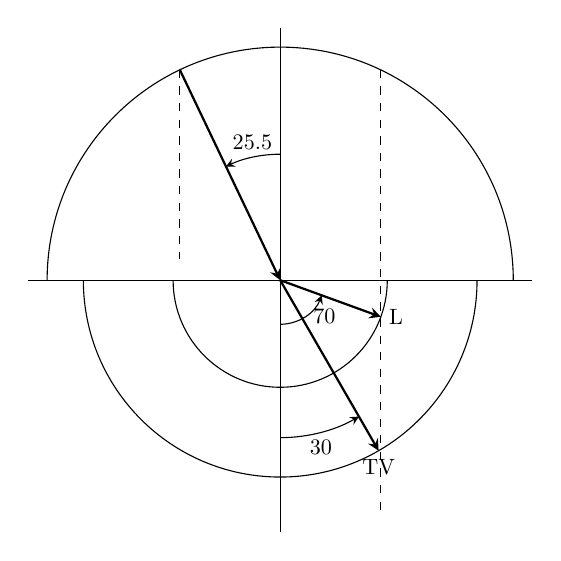
\begin{tikzpicture}[>=stealth, scale=0.8, transform shape]
        % interface
        \draw (-4,0) -- (4,0);
        \draw (0,-4) -- (0,4);

        % plexi
        \draw (3.7,0) arc (0:180:3.7); % L

        % acier
        \draw (3.125,0) arc (0:-180:3.125); % TV
        \draw (1.7,0) arc (0:-180:1.7); % L

        % incident wave
        \draw[<-, thick] (0,0) -- (115.5:3.7);
        \draw[dashed] (115.5:3.7) -- ++(0,-3);
        \draw[dashed] (64.5:3.7) -- ++(0,-7);

        % refracted
        \draw[thick, ->] (0,0) -- (-20:1.7) node[right] {L};
        \draw[thick, ->] (0,0) -- (-60:3.125) node[right, below] {TV};

        % angles
        \draw[->] (0,2) arc (90:115.5:2) node[midway, above] {25.5\degres};
        \draw[->] (0,-.7) arc (-90:-20:.7) node[midway, right] {70\degres};
        \draw[->] (0,-2.5) arc (-90:-60:2.5) node[midway, below] {30\degres};
    \end{tikzpicture}
    \caption{Cercles des lenteurs pour un angle d'incidence de 25.5\degres.}
    \label{tofd:lenteurs}
\end{figurehere}

\subsubsection{Ondes générées}

La description faîte de la méthode précédemment correspond à une transmission
latérale\footnote{\textit{Pitch \& Catch}} avec réflexion sur le fond de plaque. En
faisant ce choix il y aura, \textit{a priori}, une conversion de mode au niveau de la
réflexion, le récepteur verra donc des ondes transversales et longitudinales.
Les calculs réalisés en ~\ref{tofd:par:inc_plexi_acier} montrent qu'en réalité, compte
tenu de l'angle du sabot, des ondes transversales et longitudinales seront générées dès
l'entrée en plaque.

En effet, la méthode TOFD produit et mesure successivement trois ondes différentes en raison de l'agencement du transducteur et du récepteur :

\begin{enumerate}
    \item Une onde latérale, causée par la propagation directe, entre l'émetteur et le
			récepteur juste sous la surface de l'échantillon (voir \ref{tofd:par:laterale})
    \item Un signal LL, issu de la réflexion de l'onde longitudinale (plus rapide) en une onde longitudinale sur le fond de plaque.
    \item Un signal LT correspondant à la réflexion de la première longitudinale sur le fond de plaque avec conversion de mode.
\end{enumerate}

D'autres ondes (issues de la réflexion de la première transversales ou de réflexions
multiples) sont aussi visble mais l'expérimentateur s'assurera de choisir une fenêtre
masquant ces signaux considérés parasites.

Lors d'un balayage normal, les trois signaux apparaissent constant sans qu'aucun bruit ne
s'intercale entre elles.

Lorsqu'un défaut est présent, un signal apparaît entre l'onde latérale et le signal LL.
La profondeur de la faille peut être calculée à partir du retard entre le signal de défaut, du temps de propagation normal du signal LL et de la distance inter-transducteur.

\subsubsection{Évaluation des angles d'incidences du plexiglas vers l'acier}
\label{tofd:par:inc_plexi_acier}

Il est important de calculer les angles d'incidence et de réfraction pour les différentes interfaces afin de s'assurer des types d'ondes générés.

\paragraph{Angles critiques} D'après le tableau~\ref{table:params_tofd} et la relation de Snell-Descartes~\eqref{tofd:snell},
les angles critiques pour les ondes longitudinales et transversales sont présentés en~\eqref{tofd:crit_L} et~\eqref{tofd:crit_T}.

\begin{equation}
    \frac{\sin\theta_1}{v_1} = \frac{\sin\theta_2}{v_2}
\label{tofd:snell}
\end{equation}

\begin{equation}
    \theta_{crit_L} = \arcsin\left(\frac{\tilde{v_L}}{v_L}\right) \approx 27.23\deg
    \label{tofd:crit_L}
\end{equation}

\begin{equation}
    \theta_{crit_T} = \arcsin\left(\frac{\tilde{v_L}}{v_T}\right) \approx  57.54\deg
    \label{tofd:crit_T}
\end{equation}


\paragraph{Incidence plexiglas/acier} La documentation du sabot donne accès à l'angle de réfraction des ondes L dans l'échantillon, en l'occurence $\theta_{R_L} = 70\deg$. Afin de vérifier quelles ondes sont générées dans l'acier, il faut maintenant vérifier la valeur de l'angle d'incidence. Toujours avec la formule de Snell-Descartes, il apparaît que des ondes transversales et longitudinales sont générées (voir~\eqref{tofd:theta_i}) car $\theta_I$ est inférieur au premier angle critique.

\begin{eqnarray}
    \frac{\sin\theta_I}{\tilde{v_L}} & = &\frac{\sin\theta_{R_L}}{v_L}\notag\\
    \Leftrightarrow \theta_I & = & \arcsin\left(\frac{\tilde{v_L}}{v_L}\sin\theta_{R_L}\right)\notag\\
    \Leftrightarrow \theta_I & = & 25.47\deg \label{tofd:theta_i}
\end{eqnarray}

L'angle de réfraction des ondes transversales dans l'acier est donné en~\eqref{tofd:theta_rt}, en utilisant le même raisonement.

\begin{equation}
    \theta_{R_T} = \arcsin\left(\frac{v_T}{\tilde{v_L}}\sin\theta_I\right) = 30.64\deg
    \label{tofd:theta_rt}
\end{equation}

\begin{table*}[h]
    \centering
    \begin{tabular}{l|cc}
        Paramètre & Valeur & Unité\\\hline
        Vitesse de l'onde longitudinale dans l'acier $v_L$ & $5900$ & $m.s^{-1}$\\
        Vitesse de l'onde transversale dans l'acier $v_T$ & $3200$ & $m.s^{-1}$\\
        Vitesse de l'onde longitudinale dans le plexiglas $\tilde{v_L}$ & $2700$ & $m.s^{-1}$\\
        Vitesse de l'onde transversale dans le plexiglas $\tilde{v_T}$ & $1100$ & $m.s^{-1}$\\
        Épaisseur de la plaque $e$ & $20\cdot 10^{-3} \pm 0.1\cdot 10^{-3}$ & $m$\\
        Fréquence d'échantillonnage $F_e$ & $200\cdot 10^{6}$ & $Hz$
    \end{tabular}
    \caption{Paramètres remarquables de la manipulation.}
    \label{table:params_tofd}
\end{table*}

\subsubsection{Onde latérale et couverture}
\label{tofd:par:laterale}

En plus des ondes longitudinales et transversales, l'excitation produit aussi une onde latérale. Celle-ci se propage le long de l'interface à la vitesse d'une onde longitudinale.

Cette onde est importante notamment pour améliorer la zone de la pièce couverte par l'inspection. En utilisant cette onde latérale, il est possible d'évaluer ce qui se passe au dessus du point de croisement des faisceaux ultrasonores.

Enfin, pour maximiser la zone couverte par les faisceaux, le point de croisement est
choisi aux deux-tiers de l'épaisseur de la plaque ; l'ajustement se fait en jouant sur la distance inter-transducteurs. Le point de référence à utiliser pour cette mesure d'écartement est le point d'émergence du faisceau, symbolisé par une marque sur le sabot.

\subsection{A propos des zones mortes}

La méthode TOFD utilise les échos produits par l'interaction du train d'onde émis avec les bords de plaque et les éventuels défauts. L'émetteur excite donc le matériau avec un train d'onde assez court qui est ensuite réfléchi jusqu'au récepteur.

L'impulsion ultrasonore émise n'est pas infinement courte, elle met donc un certain temps
à être captée par le récepteur. Ce temps crée une zone dite "morte", un intervale temporel durant lequel l'impulsion masque tout autre signal (par exemple un signal diffracté par un défaut). Il y a donc des zones en haut et en fond de plaque ou les réflexions franches sur les bords de plaques masquent les défauts. La figure~\ref{tofd:deadzones} schématise ces zones.


\begin{figurehere}
    \centering
    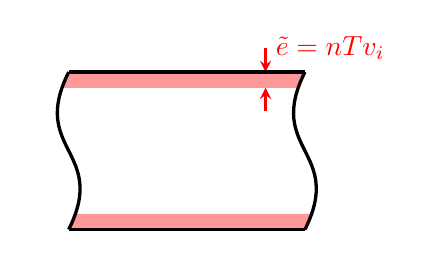
\begin{tikzpicture}[>=stealth]

        % deadzones
        \fill[red!40] (-1.5,0) -- ++(-.1,-.2) -- ++(3,0) -- ++(.1,.2) -- cycle;
        \fill[red!40] (-1.4,-1.8) -- ++(-.1,-.2) -- ++(3,0) -- ++(.1,.2) -- cycle;

        \draw[red, thick, ->] (1,.3) node[right] {$\tilde{e} = nTv_i$} -- ++(0,-.3);
        \draw[red, thick, ->] (1,-.5) -- ++(0,.3);

        % part
        \draw[very thick] (-1.5,0) -- (1.5,0);
        \draw[very thick] (-1.5,-2) -- (1.5,-2);
        \draw[very thick] (-1.5,0) .. controls (-2,-1) and (-1,-1) .. (-1.5,-2);
        \begin{scope}[shift={(3,0)}]
            \draw[very thick] (-1.5,0) .. controls (-2,-1) and (-1,-1) .. (-1.5,-2);
        \end{scope}
    \end{tikzpicture}
    \caption{Position et taille des zones mortes , $n$ désigne le nombre (\textit{a priori} rationnel) de périodes émises dans l'impulsion, $T$ la période du signal et $v_i$ la célérité de l'onde.}
    \label{tofd:deadzones}
\end{figurehere}

Plus le signal choisi pour l'inspection est haute fréquence, plus sa période est petite et par conséquent, moins les zones mortes sont larges.

\section{Mesures}

Les mesures réalisées portent sur 3 configurations.

Après la prise en main du matériel avec une configuration A scan simple (pour comprendre le concept de zone morte), deux mesures en \textit{Pitch Catch}\footnote{Transmission Latérale} sont réalisées. La première porte sur un pan de plaque sans soudur et \textit{a priori} sain, la seconde s'intéresse plus particulièrement à la soudure.

La dernière partie traite de la reproduction des expériences menées
dans~\autocite{kim_simultaneous_2003} et par conséquent la caractérisation de propriétés et géométrique de la plaque au moyen de deux mesures.

\subsection{Identification des ondes}

Afin de bien comprendre quelles ondes se propagent dans le solide, une première mesure en plaque saine est réalisée. Le A-Scan résultant est présenté en figure~\ref{tofd:ident_ondes}.

Sur ladite figure, les 3 types d'ondes présentant un intérêt pour la méthode TOFD sont présentées.
L'onde de tête (ou onde latérale) se propage le long de l'interface à la vitesse de l'onde longitudinale ; elle arrive en premier.
L'onde longitudinale arrive ensuite suivie par l'onde transversale.

\begin{figurehere}
    \centering
    \includegraphics[width=.5\textwidth]{tofd_figs/ident_ondes.png}
    \caption{Les zones encadrées correspondent chacun à une onde différente. En rouge,
		l'onde de tête se propageant le long de l'interface a la vitesse longitudinale (à
		gauche). En noir l'onde longitudinale (à droite). En vert, l'onde transversale.}
    \label{tofd:ident_ondes}
\end{figurehere}

\subsection{Mesure en plaque saine}

Un B-Scan en plaque saine est réalisé et présenté en figure~\ref{tofd:bscan_saine}. Les temps d'arrivés pour chacune des deux ondes ne changent pas tout au long du scan : cela confirme l'hypothèse d'un pan de plaque sans défaut.

\begin{figurehere}
    \centering
    \includegraphics[width=.5\textwidth]{tofd_figs/bscan_plaque_saine.png}
    \caption{B-Scan utilisant la méthode TOFD dans une plaque saine. Tout au long du scan, les ondes longitudinales et transversales arrivent toujours aux mêmes instants : il n'y a pas de défaut ou d'élément dans l'échantillon pouvant provoquer une réflexion précoce.}
    \label{tofd:bscan_saine}
\end{figurehere}

\subsection{Mesure sur la soudure}

La méthode TOFD est utilisée pour détecter des défauts dans des plaques et des cordons de soudure.

L'objectif de cette mesure est de vérifier que TOFD permet bien la détection et le positionnement de défauts (connus ici) dans un cordon de soudure.

\subsubsection{Défauts présents}

\begin{figurehere}
    \centering
    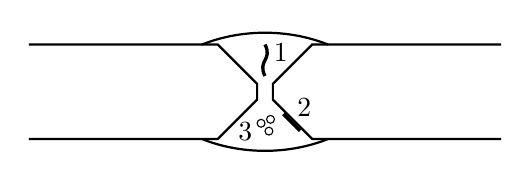
\begin{tikzpicture}
        \draw[thick] (-3,0) -- (-0.6,0) -- ++(.5,.5) -- ++(0,.2) -- ++(-.5,.5) -- (-3,1.2);
        \begin{scope}[xscale=-1]
            \draw[thick] (-3,0) -- (-0.6,0) -- ++(.5,.5) -- ++(0,.2) -- ++(-.5,.5) -- (-3,1.2);
        \end{scope}

        % center line crack
        \draw[thick] (-.8,1.2) .. controls (-.3,1.4) and (.3,1.4) .. (.8,1.2);
        \draw[thick] (-.8,0) .. controls (-.3,-.2) and (.3,-.2) .. (.8,0);

        % root fusion
        \draw[very thick] (-.05,.6) ++(-45:.4) -- ++(-45:.3);
        \draw[very thick] (0,.8) .. controls (-.1,1) and (.1,1) .. (0,1.2);

        % porosity
        \draw (.05,.1) circle (.05);
        \draw (.07,.25) circle (.05);
        \draw (-.05,.2) circle (.05);

				\node (crack) at (.2,1.1) {1};
				\node (fusion) at (.5,.4) {2};
				\node (porosity) at (-.25,.1) {3};
		\end{tikzpicture}
    \caption{Localisation des défauts au sein du cordons, coupe transversales avec projeté (reproduction depuis la documentation).}
    \label{tofd:fig:defects}
\end{figurehere}

\begin{tablehere}
\centering
\begin{tabular}{c|c|c|c}
Numéro & Type & Taille & Position \\ \hline
1 & Fissure médiane & 21 & 46 \\
2 & Manque de fusion & 25 & 147 \\
3 & Porosité & 27 & 213
\end{tabular}
\caption{\label{tofd:tab:defects} Type, position et taille (en mm) des défauts au sein de la soudure.}
\end{tablehere}

\subsubsection{Éxpérience}

Un B-Scan est réalisé le long de la soudure afin d'essayer de positionner les défauts, le
résultat est visible en figure~\ref{tofd:fig:weld}.

\begin{figurehere}
	\centering
	\includegraphics[width=0.8\linewidth]{tofd_figs/soudure.png}
	\caption{B-Scan le long de la soudure, les modifications de l'écho sont marquées en
	rouge. Ces modifications apparaissent pour $x=21mm$, $x=129mm$ \& $x=192mm$.}
	\label{tofd:fig:weld}
\end{figurehere}

L'écart entre les positions indiquées par la documentation liée à la plaque d'essai et
celles mesurées est assez important. Le manque d'expérience des manipulateurs est
probablement à blâmer et le mauvais calage de l'origine lors de la mesure n'améliore rien.

Des réflexions précoces sont toutefois bien visibles et il est possible en travaillant
mieux les aspects pratiques de la mesure d'obtenir un positionnement précis des défauts
dans une pièce.

\subsection{Caractérisation de la plaque par deux mesures}

La détermination de l'épaisseur de la plaque et de la vitesse de propagation au sein de
celle-ci est parfois complexe. Disposer d'une méthode permettant de déterminer rapidement
ces deux quantités est donc un avantage.

Comme suggéré par Kim \textit{et coll.}\autocite{kim_simultaneous_2003}, deux mesures à
deux distances inter-transducteurs différentes sont nécessaires pour accèder aux paramètres d'intérêt.

\begin{figurehere}
	\centering
	\includegraphics[width=0.8\linewidth]{tofd_figs/time_records_publi.png}
	\caption{Traces des deux signaux mesurés (attention, les abscisses ne concordent pas) pour
	la détermination simultanée de l'épaisseur et de la vitesse de propagation.}
	\label{tofd:fig:traces_publi}
\end{figurehere}

\begin{table}
	\centering
	\caption{Temps de vols et distances inter-transducteurs relevé pour la mesure
	simultannée de l'épaisseur et de la vitesse de propagation.}
	\label{tofd:tab:publi}
	\begin{tabular}{c|c}
		Distance ($mm$) & Temps de vol ($\mu s$)\\\hline
		36 & 12.25\\
		72 & 24.38\\
	\end{tabular}
\end{table}

Les signaux relevés ainsi que les temps mesurés sont présentés en
Figure~\ref{tofd:fig:traces_publi} et en Table~\ref{tofd:tab:publi}. En utilisant les
équations (3) et (4) de \cite{kim_simultaneous_2003} (reproduites en~\eqref{tofd:kim_d}
et~\eqref{tofd:kim_v}), les valeurs d'épaisseur et de vitesse de propagations sont
retrouvées (voir~\eqref{tofd:result_d} \&~\eqref{tofd:result_v}).

\begin{equation}
	d = \frac{1}{2}\sqrt{\frac{L_2^2T_1^2 - L_1^2T_2^2}{T_2^2 - T_1^2}} \label{tofd:kim_d}
\end{equation}

\begin{equation}
	v = \sqrt{\frac{L_2^2 - L_1^2}{T_2^2 - T_1^2}} \label{tofd:kim_v}
\end{equation}

\begin{equation}
	d \approx 19.4mm \label{tofd:result_d}
\end{equation}

\begin{equation}
	v \approx 2960 m\cdot s^{-1} \label{tofd:result_v}
\end{equation}

Les erreurs commises par rapport aux valeurs théoriques d'épaisseur et de vitesse sont
respectivment de 7.24\% et 7.60\%. Le fait que les deux erreurs soient si proches indique
que le facteur d'imprecision est probablement le même pour les deux. La méthode est
suffisament précise pour donner de bon résultats attendu que la mesure des temps de vol et
de la distance inter-tranducteur soit bonne.

\section*{Conclusion}

Ce TP a permis de comprendre le principe de fonctionnement de la méthode TOFD tant pour le
positionnement de défaut que pour des applications annexes de mesure d'épaisseur ou de
vitesse de propagation.

Concrètement, la force de cette méthode est sa facilité de mise en oeuvre et son faible
coût. Elle est adaptée à des applications diverses sans demander une longue formation du
manipulateur.
